%                                                                 aa.dem
% AA vers. 9.1, LaTeX class for Astronomy & Astrophysics
% demonstration file
%                                                       (c) EDP Sciences
%-----------------------------------------------------------------------
%
%\documentclass[referee]{aa} % for a referee version
%\documentclass[onecolumn]{aa} % for a paper on 1 column  
%\documentclass[longauth]{aa} % for the long lists of affiliations 
%\documentclass[letter]{aa} % for the letters 
%\documentclass[bibyear]{aa} % if the references are not structured 
%                              according to the author-year natbib style

%
\documentclass{aa}  

%
\usepackage{graphicx}
%%%%%%%%%%%%%%%%%%%%%%%%%%%%%%%%%%%%%%%%
\usepackage{txfonts}
%%%%%%%%%%%%%%%%%%%%%%%%%%%%%%%%%%%%%%%%
%\usepackage[options]{hyperref}
% To add links in your PDF file, use the package "hyperref"
% with options according to your LaTeX or PDFLaTeX drivers.
%
\begin{document} 


   \title{The variability of Betelgeuse explained by surface convection}


    \author{{ Q.~Pilate}\inst{1},{ A.~L{\'o}pez Ariste}\inst{1},{ A.~Lavail}\inst{1},{ Ph. Mathias}\inst{1} }

   \institute{IRAP, Universit\'e de Toulouse, CNRS, CNES, UPS.  14, Av. E. Belin. 31400 Toulouse, France 
             }

   \date{Received ...; accepted ...}

% \abstract{}{}{}{}{} 
% 5 {} token are mandatory
 
  \abstract


   \keywords{
               }

   \maketitle
%
%-------------------------------------------------------------------

\section{Introduction}

Betelgeuse is a prototypical red supergiant (RSG) known to be a semi-regular variable. Several periods can be found in the 
literature usually clustered around the so-called long secondary period (LSP) of 2000 days and other more or less well defined 
periods around 400 and 200 days. Such periods are often linked to radial pulsation modes,   and have been used to model 
the caracteristics of the resonant cavity, hence the size of the star and eventually its evolutionary stage \cite{XXX}.

At the end of 2019, Betelgeuse suffered a sudden and dramatic loss of brightness \cite{}, particularly in the blue colors. 
\cite{} has demonstrated that such event was due to the emission by the star of a cloud of dust near to the line of sight of 
Earth. In this event it was clear that a change in brightness was not due to any kind of pulsation but to a change on the 
brightness distribution over the stellar disk due to the presence of large quantities of dust. While this may be seen as 
a singular event, it brings up the question whether all changes in brightness cannot be due to similar changes in the brightness 
distribution over the disk. 

Betelgeuse is known to present large convective cells with life times in the order of one to two years and measurable changes 
in the span of one week. Bright convection cells near disk center will increase the integrated brightness of the star when 
compared with other situations where such cells are found near the edges. So even without calling for the formation of 
dust or other changes in opacity, one may argue that the simple convective patterns of the star may create a variability. Such 
variability could be expected to be random, but will present quasi-periodicities related to the typical time scales of the 
convective patterns. 

Since the end of the Great Dimming event, Betelgeuse has continue its random variation of brightness. But the classical periods 
of variation cited above are not visible any more. This may be due to simply the short span of time, that does not afford for 
the peaks to appear prominently in the variability spectra. But it has been sufficient to bring up that other explanation of the variability
in terms  of convective patterns. In order to address this question we seek for the typical periods of 1000, 400 and 200 days in  
observational proxies related to the convective activite but unrelated to pulsations nor directly linked to brightness?

Linear polarization in the atomic lines of the spectra of Betelgeuse, discovered by \cite{}, has been interpreted as the joint action of 
two mechanisms. First the depolarization of the continuum by atoms which absorb linearly polarized light and re-emit unpolarized light, the 
continuum photons being polarized by Rayleigh scattering. This depolarization produces signals with an azimuth symmetry over the disk that 
would  cancel out the net linear polarization on a homogeneous disk. Thus it must be combined with an inhomogenous disk to produce the net linear polarization 
signal observed. This interpretation suggested the possibility of mapping those brightness inhomogeneities. This has been done by \cite{} 
even producing 3-dimensional images of the atmosphere of Betelgeuse \cite{} when taking advantage of the different height of formation of 
different lines in the spectrum of Betelgeuse. The images produced compare very well with cotemporaneous images made with interferometric 
techniques and show clear convective patterns. Linear polarization in the atomic lines is therefore a proxy of convection, unrelated to radial 
pulsations but linked to the brightness inhomogeneities due to the convective patterns in Betelgeuse. If one can find the aforementioned periods 
in linear polarization, we must conclude that these periods are related to the convective activity which originates those linear polarization 
and unrelated to any radial pulsation phenomena.




Betelgeuse is a red super giant star which has been observed by many astronomers for centuries. This star is known as a 
semi variable star. In the literature, the variability of the light curve of Betelgeuse is mainly explained by pulsation of 
the atmosphere. The most common periods found in Betelgeuse are the long secondary period (LSP) which is around $2000$ days 
and there are few known overtones such as $400$ days or $200$ days. Since the great dimming between the end of 2019 and 
beginning of 2020, those periods have changed. In this article, we attempt to recover the different periods of Betelgeuse 
using surface convection. The brightness of Betelgeuse is linked to the giant convective cells present at the surface. Hence, 
the light curve will be affected by the size and the number of convective cells at the surface and also by the timescale on 
those convective cells live. To explain to variability of Betelgeuse, we used the polarimetric data from the telescope Bernard 
Lyot, which observed Betelgeuse over a decade almost weekly. The linear polarization in Betelgeuse is associated to brightness 
inomogeneities at the surface of the star, due to huge convective cells at the surface. From the linear polarization signal, 
we were able to produce images of Betelgeuse. From the variability of the linear polarization and the intensity signal, we 
attempted to recover the variability of Betelgeuse. We also tried to recover the variability using the images produced by 
polarimetry. The photo-center displacement is affected by the size, number and timescale of convective cells. Using our 
images, we followed the displacement of the photo-center of Betelgeuse over 10 years to recover the variability of 
Betelgeuse. 

\section{Method}

Trying to find periods in an astrophysical context can be difficult due to the unevenly spaced observed data. To overcome this issue, we used the Lomb-Scargle (LS) periodogram. For a given set of data, it fits a periodic signal using least squares method, for each frequency between the first and the last observation. The better the periodic signal fits the data, the higher the power attributed to the frequency. We used the LS periodogram in the linear polarization ($\sqrt{Q^2+U^2}$) and intensity signal first. 

\begin{figure}[!h]
    \centering
    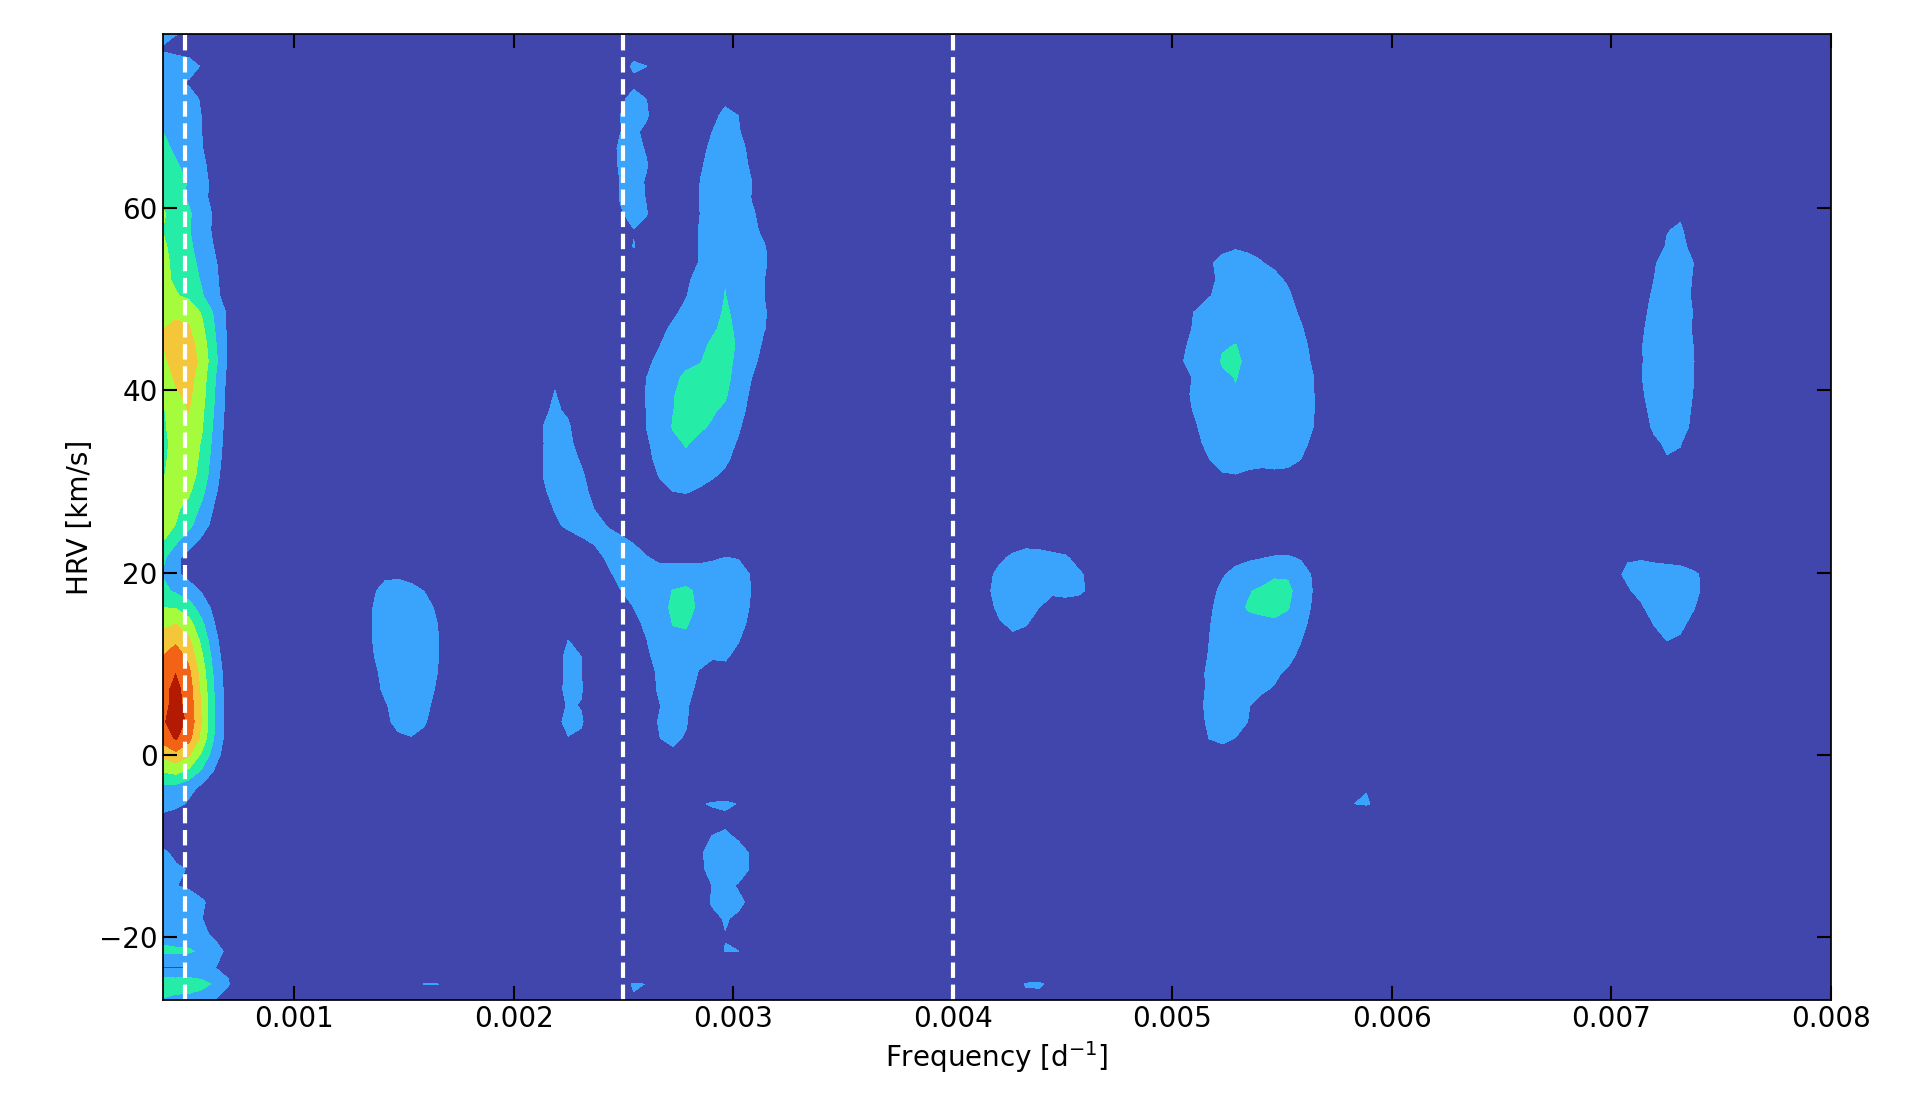
\includegraphics[width=0.5\textwidth]{LS Intensity.png}
    \caption{Lomb-Scargle periodogram of intensity over 10 years. Red regions represent high LS power (i.e most plausible frequencies) whereas blue regions stands for low LS power. }
    \label{LS Intensity}
\end{figure}

Figure \ref{LS Intensity} shows the LS periodogram of intensity for each frequency between -25 km/s and 70 km/s. The white dashed lines reprent the three main sequences found in the literature i.e the LSP and its overtones at 400 days and 250 days. From the intensity signal, we recover the LSP around 2000 days. For lower frequencies (i.e periods higher than 2000 days), the signal is attributed to cross correlation. It appears that there is a small signal around $0.003 d^{-1}$ ($\sim 333$ days) but it is hard to affirm that it corresponds a net signal or noise. \\

Figure \ref{LS Pl} shows the LS periodogram of linear polarization. We see that we find a strong power around a period of 400 days (second dashed line). In the linear polarization, the LSP does not appear in the LS periodogram. Hence, from the intensity and the linear polarization signal, we recover two of the three main periods found in Betelgeuse.Interestingly, the period around 250 days is present in the LS periodogram of stokes Q (see figure \ref{LS Q}) but not in stokes U. The nature of the differents periodicity is discussed in the next section, especially the one found in the linear polarization. 


\begin{figure}[!h]
    \centering
    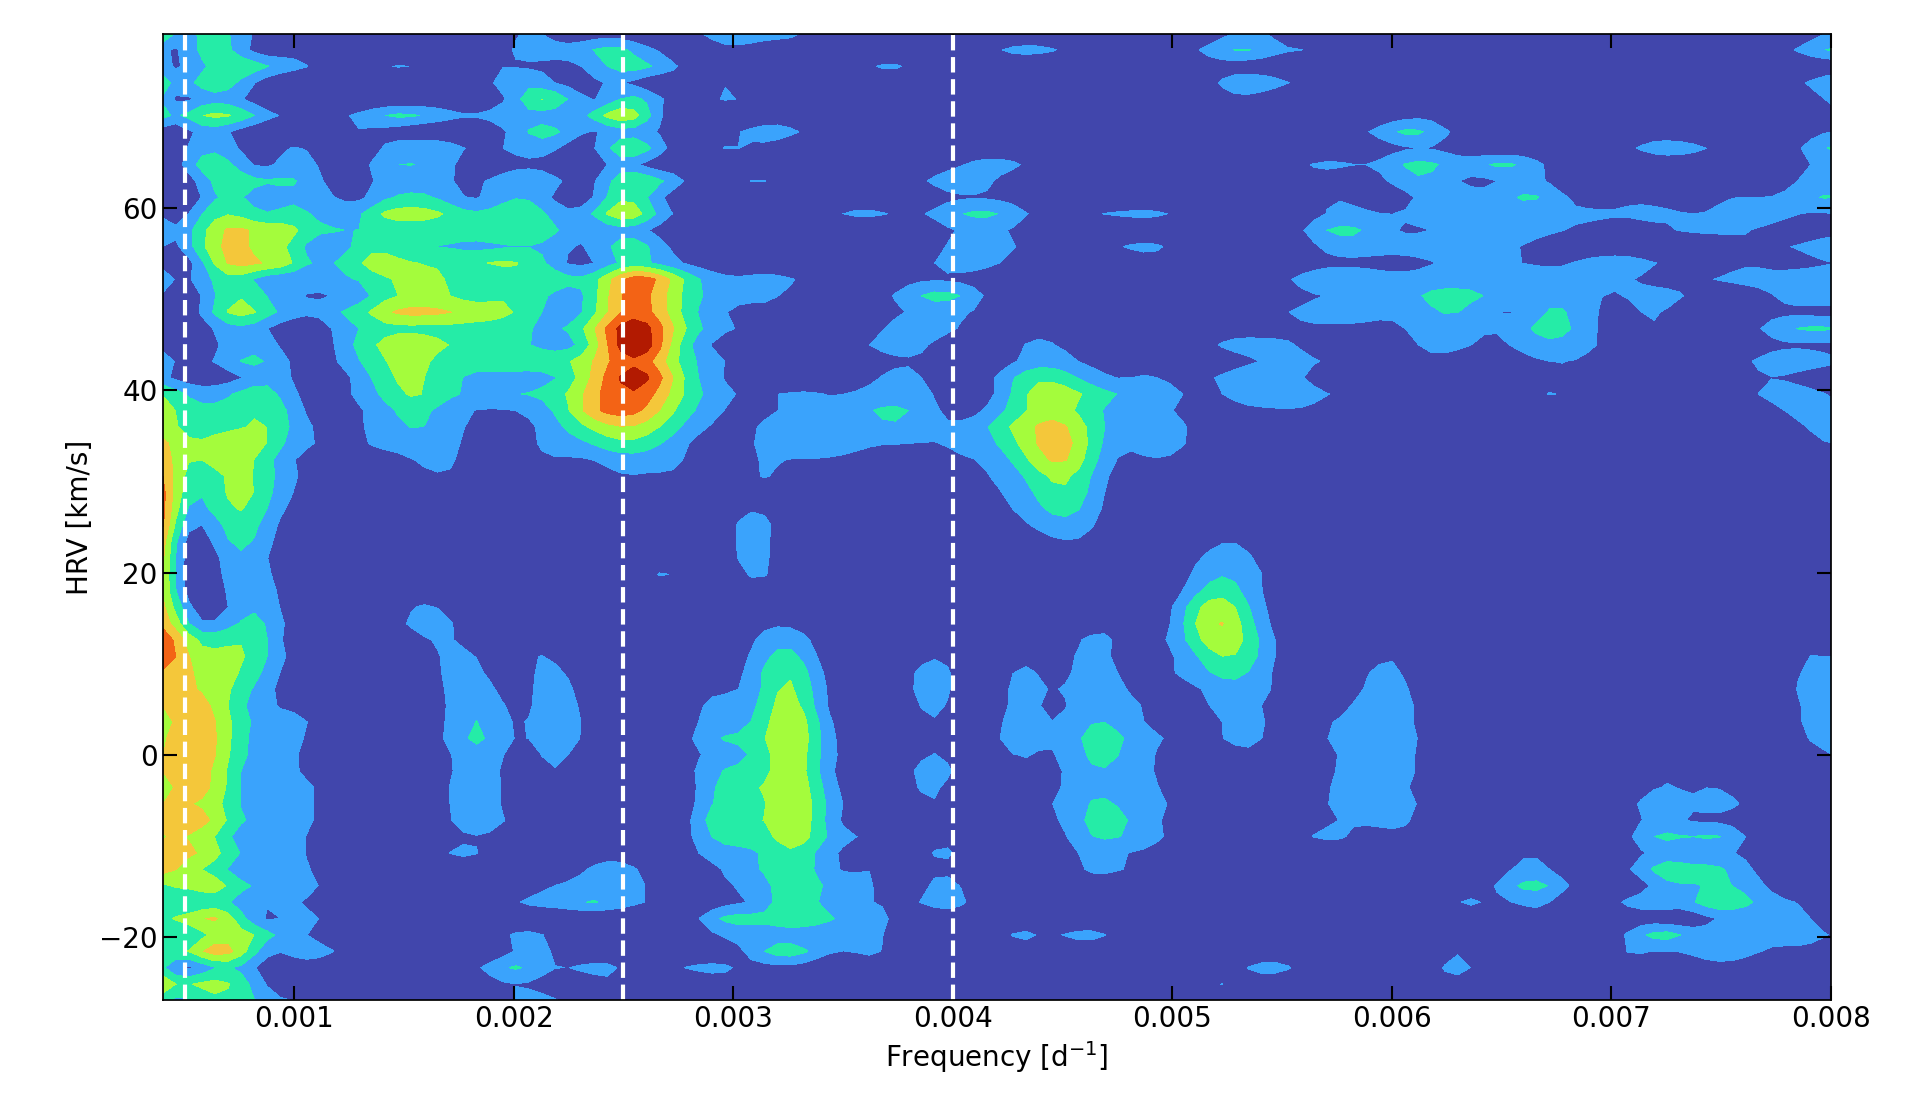
\includegraphics[width=0.5\textwidth]{LS Pl.png}
    \caption{Lomb-Scargle periodogram of linear polarization. The colour code is the same as figure \ref{LS Intensity}. }
    \label{LS Pl}
\end{figure}

\section{Convection to explain periodicities}

In the previous section, we have seen that we recover the different periods of Betelgeuse from the intensity and linear polarization signal. While the nature of the LSP is still in debate, the nature of the lower periods is attributed to pulsation of the atmosphere of Betelgeuse. However, the mechanism behind the pulsation of Betelgeuse is less clear. In this section, we attempt to find an explanation to the 400 days periodicity of Betelgeuse. As mentioned before, the LS periodogram of linear polarization shows a periodicity around 400 days. Furthermore, the region where the LS power is high is around a wavelength of 40km/s. This wavelength correspond to the red wing of Betelgeuse. The polarization signal is supposed to stand between -20 and 40km/s. Signal above 40km/s is associated to plasma rising behind the limb of Betelgeuse. Hence, the strong power associated at this wavelength might be due to those convective plumes that are rising above the limb from time to time. From this scenario, we can explained the 400 days period in the light curve as follow: from time to time, Betelgeuse is ejecting plasma in the interstellar medium. Sometime, the plasma is ejected behind Betelgeuse, but rises so high that we can see the rising plume from Earth. This plume increases the number of photons that come to the Earth, leading to an increase of the brightness. After a few weeks or months, the plumes fall back to Betelgeuse, decreasing the brightness of Betelgeuse. This would explain why we recover the 400 days periodicity from linear polarization. 




\begin{figure}[!h]
    \centering
    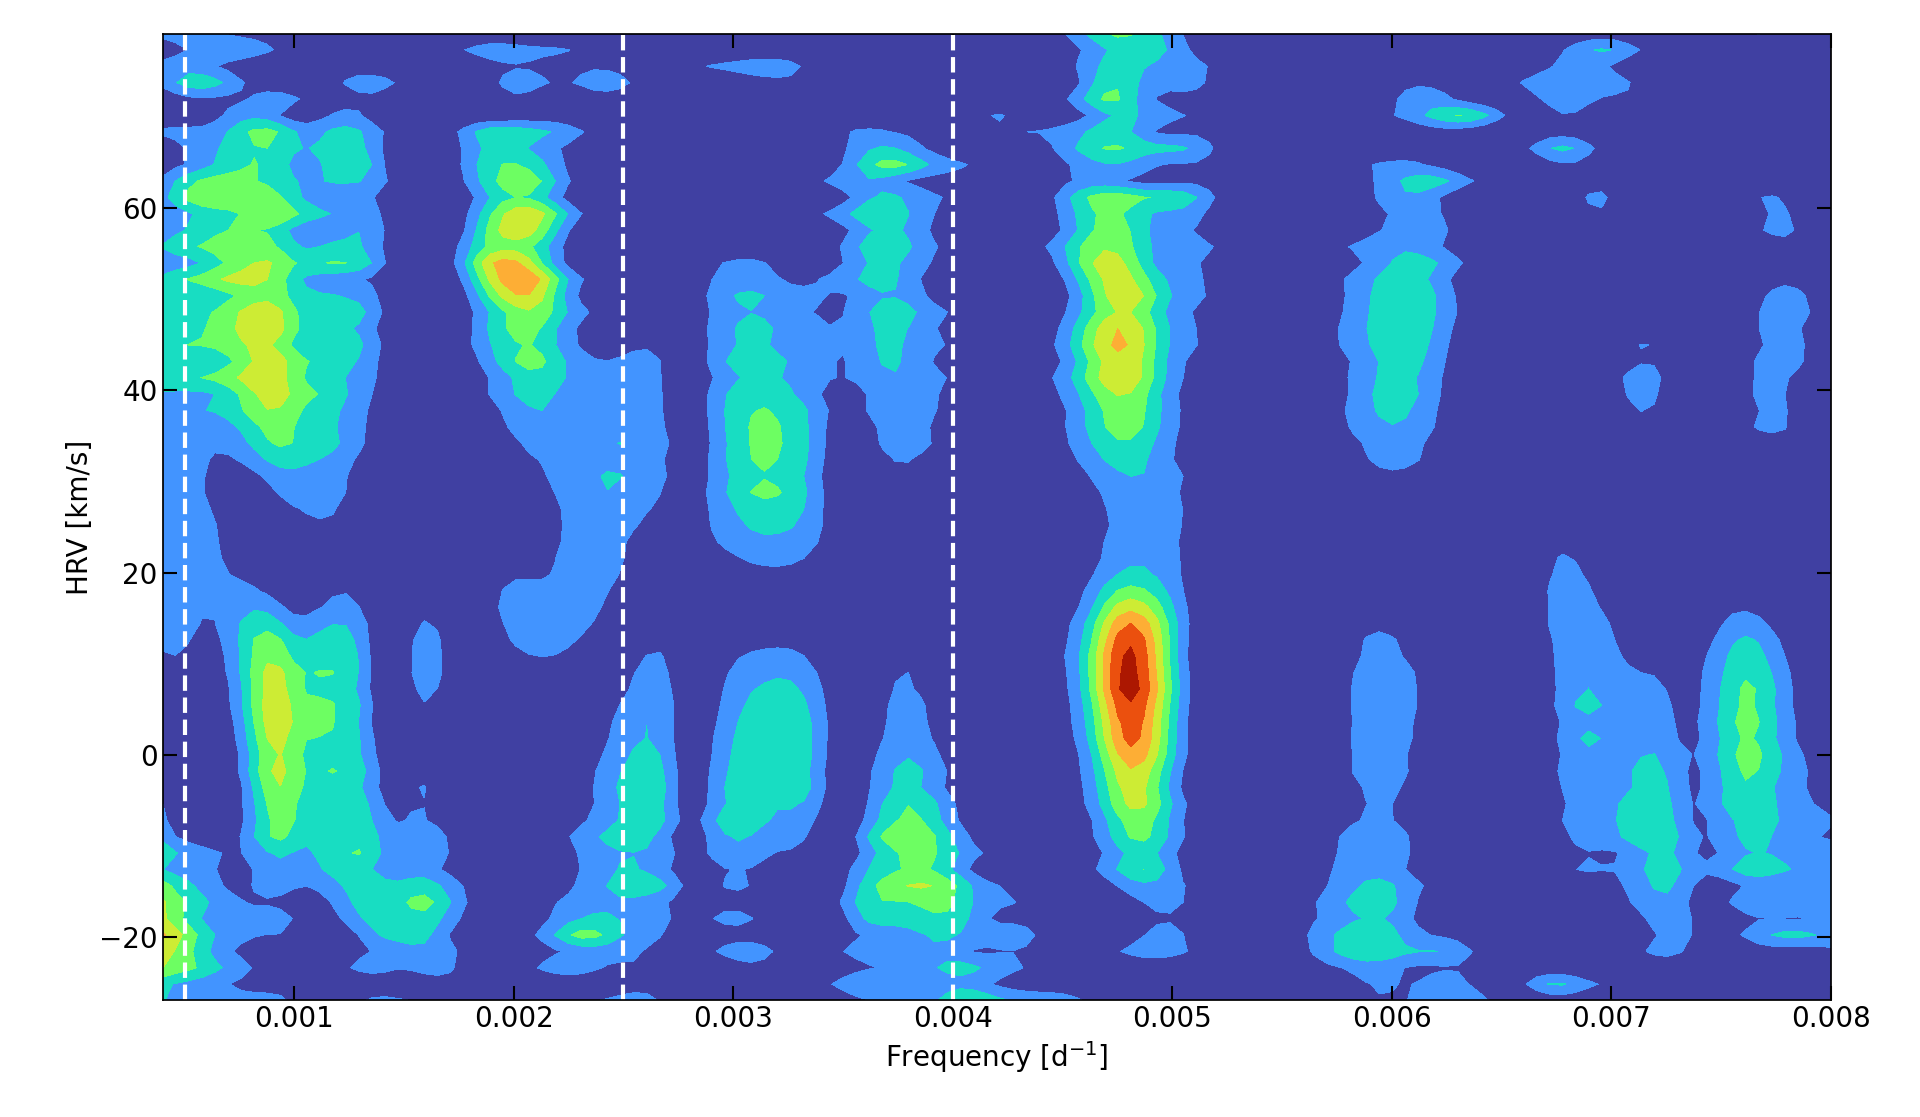
\includegraphics[width=0.5\textwidth]{LS stokes Q.png}
    \caption{stokes Q}
    \label{LS Q}
\end{figure}



\end{document}


